\documentclass[letterpaper,10pt,conference]{ieeeconf}
\IEEEoverridecommandlockouts
\overrideIEEEmargins
\usepackage[T1]{fontenc}
\usepackage{times}
\usepackage{graphicx}
\usepackage{amsmath,amssymb}
\usepackage{booktabs,tabularx,array}
\usepackage{cite}
\usepackage{flushend}
\usepackage[hidelinks]{hyperref}
\graphicspath{{figures/}{../assets/code_as_learning_machine/}}
\newcommand{\system}{RoboEvolve}
\newcommand{\SE}{\mathrm{SE}(3)}
\newcommand{\SO}{\mathrm{SO}(3)}
\newcommand{\ap}{a}
\newcolumntype{Y}{>{\raggedright\arraybackslash}X}
\hypersetup{pdfauthor={},pdfsubject={Laboratory robot manipulation}}
\pdfinfoomitdate=1
\pdftrailerid{}
\begin{document}

\title{Learning to Open and Remove:\\Evolving Robot Control Code for Laboratory Manipulation}
\author{Anonymous Authors}
\maketitle
\thispagestyle{empty}\pagestyle{empty}
\begin{abstract}
Opening laboratory equipment and removing a container cap require more than
reaching and closing a gripper. The robot must change an object's constraint
while distinguishing successful release from loss of contact. We study how a
human-guided coding agent acquires these operations by revising executable
perception, control, and verification code from physical feedback. Two case
studies use a shared laboratory robot stack but different action supervision.
For an incubator door, twelve successful teleoperation episodes selected from
57 candidates are compiled into a contact-relative trajectory with depth-based
orientation alignment and grasp checks. For a culture-media bottle cap, no
cap-specific teleoperation demonstration is supplied; one target click and
seven calibration observations support a local visual controller. Recorded
results show a verified open-door endpoint, a separate verified closing run,
and cap removal followed by 107.4\,mm of held transport. Failed and successful
door pulls both end with nearly closed, empty jaws, demonstrating why gripper
state alone is an inadequate task evaluator. The contribution is an auditable
account of how physical failures changed the representation and verification
of manipulation, not a benchmark-wide success-rate claim. The resulting
controllers execute without a language model in the servo loop.
\end{abstract}

\section{Introduction}
An incubator door and a bottle cap are small obstacles to an automated
biological workflow, yet each exposes a gap between robot motion and useful
physical work. A gripper can close without engaging a recessed handle. It can
briefly retain contact and then slide off. A cap can appear to rise because
the entire bottle moved. A command trace that looks correct is therefore not
enough: the robot must verify what changed in the world.

We call the common structure \emph{constraint-release manipulation}. The
robot engages an object, moves it relative to a supporting body, and establishes
a new access state. A door remains constrained by its hinge but leaves the
closed configuration. A cap separates from the bottle opening and must remain
held afterward. This definition groups the tasks by their required state
transition; it does not assume a measured break-away force, a particular latch,
or a threaded cap.

The central challenge is that evidence of grasping and evidence of task
completion can disagree. In our door trials, both failed pulls and successful
opening endpoints were followed by an almost fully closed gripper. The same
signal meant that contact was absent, but did not reveal whether the door had
opened. Conversely, a partially closed gripper did not prove that the cap had
separated from a stationary bottle. These ambiguities motivated changes to
the code that acquires observations, selects motion, and judges outcomes.

\begin{figure}[t]
\centering
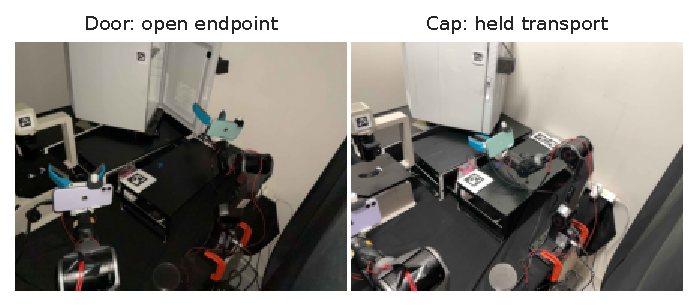
\includegraphics[width=\columnwidth]{task_overview.pdf}
\caption{Two laboratory access operations. Left: the door is open at the
verified endpoint of T7. Right: the cap remains held after transport, with the
bottle mouth exposed. Images show outcomes, not repeated trials.}
\label{fig:overview}
\end{figure}

Coding agents offer a way to revise these mechanisms together. Instead of
only modifying action-network weights, they can inspect images, mine archived
demonstrations, fit geometric models, write numerical controllers, and change
when a trial is allowed to continue. We investigate this process in an existing
laboratory cell, with human task instructions and intermittent corrections.
The agent was not given a finished door-opening or cap-removal policy. It was
given a working robot repository and access to observations and tools.

Our contribution has three parts. First, we formulate the distinction between
\emph{engagement}, \emph{release}, and \emph{retention} as explicit evidence
requirements. Second, we describe two executable controllers assembled through
physical feedback: demonstration-grounded door manipulation and cap removal
without a task-specific action demonstration. Third, we reconstruct the
failure-to-code-change chain using saved observations, source history, and
runtime records. This is a retrospective two-case study, not a controlled
comparison against alternative learning algorithms.

\section{Related Work}
\textbf{Laboratory automation.} A mobile robotic chemist demonstrated how a
robot can operate conventional laboratory equipment within an autonomous
experimental search~\cite{chemist}. Our focus is earlier in that pipeline:
acquiring and validating the small manipulation capabilities that make
equipment and containers accessible. We optimize neither an assay nor a
biological hypothesis in these experiments.

\textbf{Code-generating robot agents.} Code as Policies composes executable
robot behavior from language-generated programs~\cite{cap}. VoxPoser combines
language-guided spatial reasoning with model-based trajectory generation and
can incorporate contact experience~\cite{voxposer}. ReAct exemplifies the
broader reasoning--action feedback pattern~\cite{react}. We focus on how
physical failure changes a persistent controller and its evidence requirements,
rather than on a single generated plan.

\textbf{Physical policy improvement.} ENPIRE constructs reset and verification
interfaces through human-guided coding agents, then exposes fixed environment
APIs for autonomous policy improvement~\cite{enpire}. It supports heuristic,
imitation, reinforcement-learning, and hybrid approaches. Our study shares the
physical feedback premise; it examines laboratory access operations and traces
changes to observation and verification alongside control. We do not claim
that tool use or agent-generated environment code is absent from ENPIRE.

\textbf{Learned motor policies.} OpenVLA and $\pi_{0.5}$ demonstrate the value
of pretrained visuomotor policies and broad generalization~\cite{openvla,pi05}.
Our cap result uses zero \emph{cap-specific} action demonstrations and no
task-specific neural-policy training; it does not imply that VLAs require a
new demonstration for every deployment. Program adaptation is complementary:
a learned motor policy could be one component of the same execution stack.

\textbf{Perception and simulation.} SAM provides general-purpose segmentation
~\cite{sam}, while MuJoCo supports model-based kinematics and contact analysis
~\cite{mujoco}. Both were available in the broader development environment.
The two accepted runtime paths instead used classical image operations,
registered depth, and mechanical state for their critical evidence. The
relevant capability was selecting suitable tools, not maximizing their number.

\section{Task and Evidence Model}
\subsection{What must change?}
Let $o_t$ contain images, depth, and measured robot state. Let $g_t$ denote
engagement evidence, $r_t$ a task-specific release state, and $h_t$ continued
retention. These are predicates over observations, not synonyms for issued
commands. The cap goal requires $r_t\land h_t$: removal without dropping the
cap. The door goal requires an independently observed open state; continuous
handle retention is desirable but not necessary to label the final door state.

This distinction changes recovery. An empty grasp after a pull cannot safely
trigger another identical pull without first inspecting the door. Similarly,
opening the jaws at a destination does not establish stable cap placement. The
program must stop the claim at the last supported stage.

\subsection{Development and execution are separate loops}
During development, Codex reads observations and code, proposes a revision,
and tests a bounded physical segment. The operator supplies task intent and
semantic or geometric corrections when needed. Successful behavior is retained
as an executable artifact with configuration and tests. During execution, a
deterministic state machine calls camera, geometry, and motion interfaces; it
does not ask the language model to produce every servo command.

We represent a development artifact as $C=(P,V,X)$, where $P$ specifies target
interpretation and motion, $V$ specifies evidence checks, and $X$ connects
observation and execution services. A physical failure can require a change to
any of these, not just a numeric gain. For example, replacing a shadow-based
feature changes $P$; adding a door-state check changes $V$; isolating a fragile
camera process changes $X$.

\begin{figure}[t]
\centering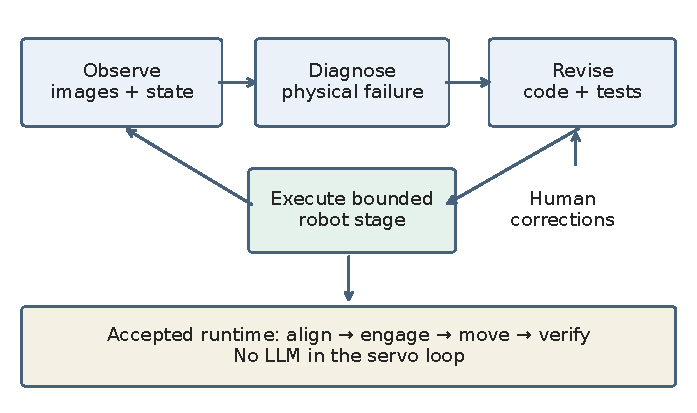
\includegraphics[width=\columnwidth]{learning_loop.pdf}
\caption{Development changes executable code; deployment runs the resulting
controller. Human corrections enter development. Saved physical observations
remain separate from editable code and retrospective analysis.}
\label{fig:loop}
\end{figure}

\subsection{Resources and supervision}
The system used a bimanual Piper installation with a position-controlled
gripper, fixed-head Record3D RGB-D, and RGB wrist cameras. The reported
manipulation used the right arm. The existing repository supplied robot RPC,
CAN control, forward/inverse kinematics, gripper calibration, and camera
interfaces. MuJoCo/Mink supplied model-based checks; fixed fiducials supported
camera registration. The agent also had shell, Python, numerical libraries,
tests, version history, and prior development context.

\begin{table}[t]
\caption{Action supervision and additional resources. A demonstration is an
episode, not a single pose.}
\label{tab:resources}\centering\small
\begin{tabularx}{\columnwidth}{lYY}\toprule
Resource & Door opening & Cap removal\\\midrule
Task action demos & 12 successes selected from 57 archived episodes & 0 cap-specific episodes\\
Human input & Task instruction, archive location, corrections & One target click, semantic/geometric corrections\\
Physical data & Contact, proof, pull, endpoint observations & Seven calibration poses; approach, lift, transport observations\\
Shared tools & RGB-D/RGB, robot state & OpenCV, MuJoCo/Mink\\
\bottomrule\end{tabularx}
\end{table}

The operator explicitly introduced the archived door recordings before their
use. The agent selected successful examples and compiled them; it did not
request newly recorded demonstrations in this experiment. Door closing used a
separate closing demonstration. Cap development used no cap-specific action
trajectory but did use physical data and human feedback. Thus neither case is
data-free or human-free. Their commonality is the development mechanism, not a
claim that the completed door controller was transferred to the cap.

\section{Demonstration-Grounded Door Manipulation}
\subsection{From recordings to a contact-relative pull}
Twelve archived teleoperation episodes were accepted after inspection of
terminal head images. The compiler chose an actual medoid episode using contact
position and orientation, rather than averaging incompatible trajectories.
Its demonstrated contact pose $T_c^d$ defines a relative motion:
\begin{equation}
 \Delta T_k=(T_c^d)^{-1}T_k^d,\qquad
 T_k^{\mathrm{run}}=T_c^{\mathrm{run}}\Delta T_k.
\label{eq:relative}
\end{equation}
The selected motion contained 148 samples from closure to release, spanning
approximately 4.93\,s in the recording. The live contact anchor therefore
changes the trajectory's placement without replacing its articulated shape.
Demonstration-derived visual/pose pairs also supported a local correction
model. Demonstrations supplied motion structure, not a complete success test.

Initially, the live starting pose was incorrectly treated as a contact
reference. Saved observations exposed a large offset. The accepted approach
instead used a demonstrated pre-close pose, a current door-plane orientation,
and a bounded visual correction. Eight head RGB-D frames supported vertical
plane fitting with RANSAC; the measured yaw was compared with a reference yaw.
The right-camera red appliance label served only as an auxiliary rigid-body
feature, not as the recessed handle itself. Corrections were limited to three
steps of at most 15\,mm each. A dark, claw-like feature was rejected after the
operator identified it as a shadow.

\subsection{Engagement before sustained pulling}
At contact, the controller closed once and sampled measured gripper opening
at 20\,Hz. Opening is normalized as $a=1$ for open and $a=0$ for closed. It is
not pressure. The settled closure had to exceed the empty-grasp bound 0.02 and
remain stable over the final ten samples. A 5\,mm proof pull then tested whether
at least 65\% of the closure opening remained, followed by a stationary
reverification. A short proof reduced obvious empty pulls but was not assumed
to guarantee long-horizon retention.

For the full pull, end-effector targets were sent through the established
teleoperation command path at 30\,Hz. The accepted implementation used twice
the demonstration duration and checked opening every 15 frames. This was a
position-target controller, not a break-away force estimator. If opening fell
below the full-pull retention threshold, motion stopped, the arm retreated
15\,mm, and the jaws opened. The controller then observed the door rather than
blindly attempting another pull.

\subsection{Verifying the object, not just the gripper}
The endpoint evaluator registered head RGB-D to stored open and closed
references using fixed tags. It compared depth evidence in a door-state region
and allowed an unknown outcome when evidence was insufficient. Arm pixels
contaminating that region motivated a subsequent mask correction. References
and observations were kept distinct from the policy's expectation of success.

A separate close demonstration was necessary. Reversing the opening path
missed the effective push location by about 15\,cm in height. The accepted
closing routine used an open-jaw push from the dedicated close recording,
then checked the closed endpoint. Opening and closing share an appliance but
need not share a reversible contact policy.

\section{Cap Removal Without an Action Demonstration}
\subsection{Grounding target, jaws, and supporting bottle}
Global white-object detection confused the cap with gripper and laboratory
components. One operator click anchored the intended instance. OpenCV color,
connected-component, and geometric operations then represented a small white
cap above the colored bottle neck. Jaw midpoint and jaw span provided a
gripper-relative target geometry. Registered RGB-D localized the selected
surface, while a completed bottle/cap model represented geometry not fully
visible in depth.

The supporting bottle was recessed between platforms rather than standing on
the assumed tabletop. This changed approach ordering: align laterally in free
space, then descend, then close. MuJoCo/Mink checked candidate motion against
the scene and robot geometry. Simulation was a critic, not ground truth: one
model-only collision disagreement was later scoped to the exact route already
supported by hardware evidence, rather than disabling collision checks for
new paths.

\subsection{Learning a local image-to-motion correction}
Seven open-jaw physical observations supported a local correspondence between
robot displacement and image error. With jaw-relative error $e$ and Cartesian
displacement $\Delta x$, the controller used a local linear model
\begin{equation}
 \Delta e\simeq J\Delta x,\qquad \Delta x=-J^+e,
\label{eq:jacobian}
\end{equation}
with bounded corrections and fresh observations. This calibration learned a
local control relationship, not a general visual policy. The final waypoint
sequence preserved the physically checked approach and egress.

Before lift, the target had to lie within the jaw segment and within 0.25 jaw
spans perpendicular to it. Opening had to lie in the calibrated non-empty band
$[0.10,0.40]$. The colored bottle support could move by no more than 0.10 of
its visual scale. These normalized image checks avoided defining success by a
fixed pixel count, although the detector remained specific to the enrolled
scene and appearance.

\subsection{Removal and retention require different witnesses}
The removal check combined measured vertical rise, persistent opening, visible
jaw motion, limited bottle displacement, and reduced cap-like appearance at
the source. The transport check added measured displacement and aperture
stability. A commanded release was not accepted as placement without evidence
of a stable destination support. This separation prevented an unverified final
step from invalidating, or being confused with, the verified earlier capability.

\begin{figure*}[t]
\centering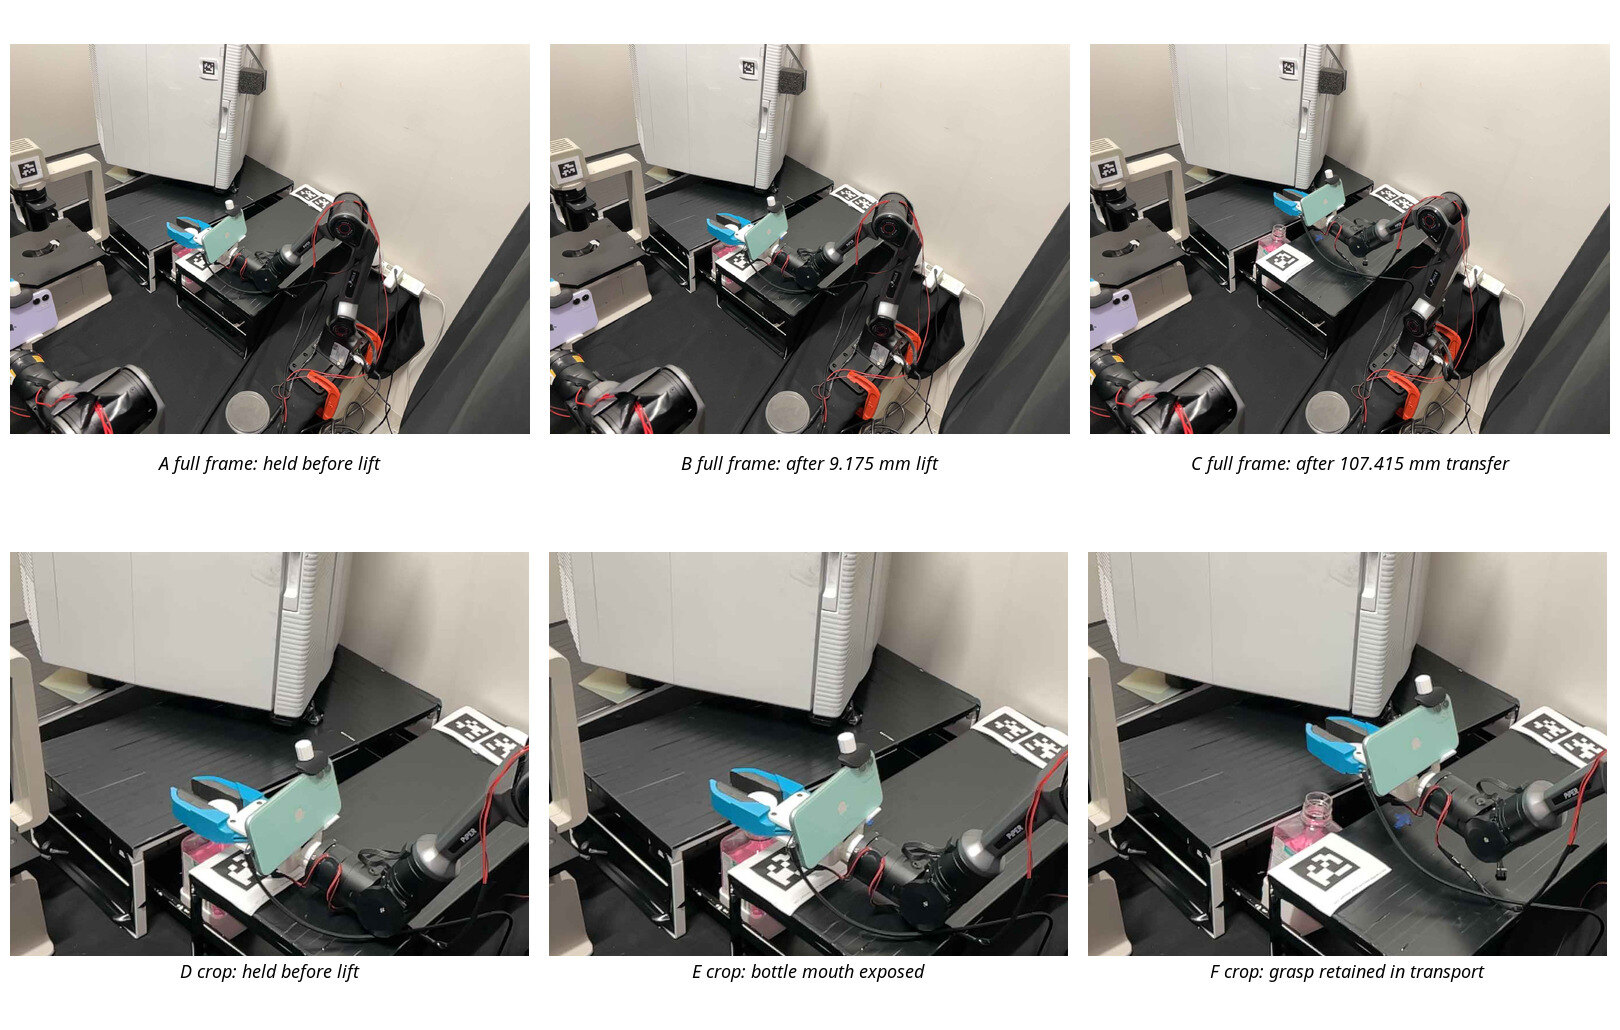
\includegraphics[width=.93\textwidth]{cap_verified_transfer_rgb.jpg}
\caption{One cap sequence, not three repetitions. Top: full fixed-head
observations before lift, after lift, and after held transport. Bottom:
corresponding detail crops. Measured end-effector rise was 9.17\,mm; subsequent
transport was 107.42\,mm. Source appearance and bottle stability complement
robot state, because end-effector motion alone does not prove cap removal.}
\label{fig:cap}
\end{figure*}

\section{Recorded Results and Failure Analysis}
\subsection{Protocol and unit of evidence}
We retrospectively aligned source revisions, command records, and immutable
observations. For the door, E1--E3 are early contact-only attempts and T1--T7
are physical pull attempts, not code versions. For the cap, the principal
quantitative result is one before-lift/after-lift/after-transport capture triplet.
The record does not contain a randomized repetition study. We therefore report
observed endpoints and measured changes, not a success-rate estimate from
these selected development records.

\begin{table}[t]\centering\small
\caption{Door opening observations. $a_c$: settled closure; $a_p$: proof
summary; $a_e$: later empty-grasp observation. Missing values are not filled.}
\label{tab:door}
\begin{tabular}{lrrrl}\toprule
Trial & $a_c$ & $a_p$ & $a_e$ & Endpoint evidence\\\midrule
T1 & .412 & .366 & .003 & Closed\\
T2 & .407 & .365 & .003 & Closed\\
T3 & .366 & .366 & -- & Not classified here\\
T4 & .323 & .319 & .004 & Not classified here\\
T5 & .293 & .291 & -- & Not classified here\\
T6 & .407 & .290 & .003 & Open observed\\
T7 & .306 & .296 & .003 & Open verified\\\bottomrule
\end{tabular}
\end{table}

\subsection{A non-empty proof did not predict the endpoint}
\begin{figure*}[t]
\centering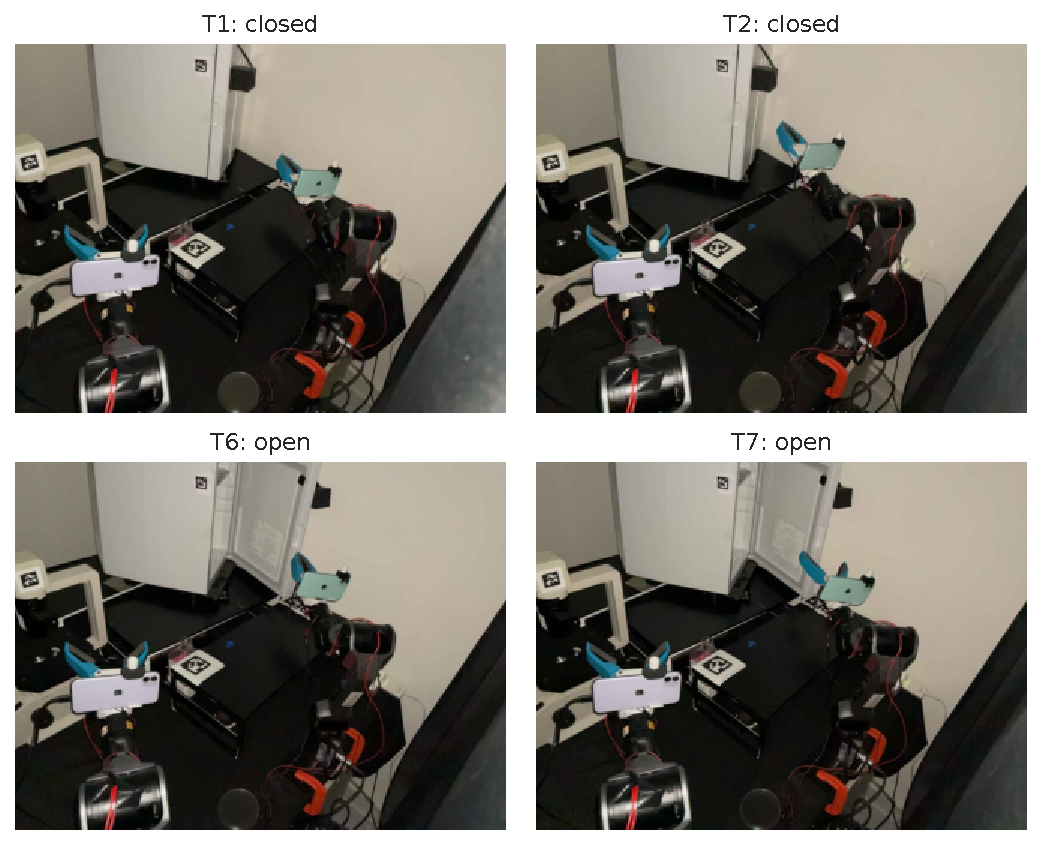
\includegraphics[width=.80\textwidth]{door_endpoints.pdf}
\caption{Saved head views for the four compared door pulls. The upper row
shows closed endpoints (T1/T2); the lower row shows open endpoints (T6/T7).
These images are acquired after the pulls, not at matched intermediate times.
The distinction remains visible even though all four later grasp observations
indicate almost closed jaws.}
\label{fig:door-images}
\end{figure*}
The first structured door pull, T1, retained opening from 0.412 after close to
0.366 after the proof. Yet its endpoint did not support opening. T2 showed a
similar pattern. Slower execution and checkpoints made subsequent failures
detectable but did not by themselves establish success. Later yaw-aligned T6
and autonomous T7 reached open endpoints, although grasp was absent afterward
(Table~\ref{tab:door}). The exact instant at which opening and slip occurred
relative to each other is not reconstructed from the sparse record.

\begin{figure}[t]
\centering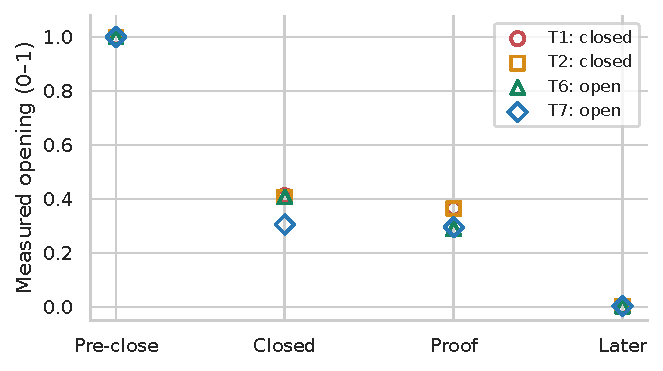
\includegraphics[width=\columnwidth]{aperture.pdf}
\caption{The same final aperture accompanies different door outcomes.
Each dot is a saved phase observation or summary; horizontal position is not
time. No full-pull curve is reconstructed. Outcome labels use later images
and depth, not aperture.}
\label{fig:aperture}
\end{figure}

T7 began from a verified closed state. Its live plane yaw was $-4.61^\circ$,
giving approximately $0.775^\circ$ residual correction relative to its
reference; one visual correction was approximately 3.5\,mm. After proof and
stationary recheck, the full pull stopped on an empty-grasp observation. The
registered endpoint was open. A separate autonomous closing run subsequently
verified the closed state. This establishes the recorded access-state changes,
not continuous grasp throughout opening or reliable repeated cycling.

\subsection{Contact orientation changed late in development}
Figure~\ref{fig:angle} compares each saved contact orientation with T7. For unit
quaternions, the distance is
\begin{equation}
 d_R(q_i,q_7)=2\arccos\!\left(\min(1,|q_i^\top q_7|)\right).
\end{equation}
The plot is a retrospective diagnostic: T7 is selected after observing success,
and its zero is true by definition. Earlier attempts are approximately
$8$--$10^\circ$ away; T6 is $2.39^\circ$ away. This is consistent with the
recorded orientation correction, but is not an isolated ablation of yaw or an
object-relative error measurement. Door pose changes are not compensated.

\begin{figure}[t]
\centering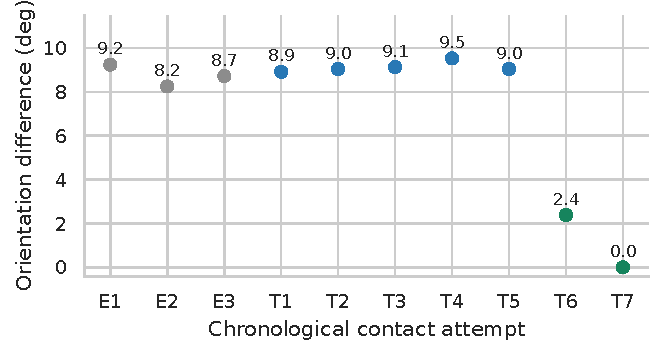
\includegraphics[width=.94\columnwidth]{orientation.pdf}
\caption{Full contact-orientation difference to successful trial T7. Gray:
early contact-only attempts; blue: T1--T5; green: T6/T7 open endpoints. T7 is a
post hoc reference, not a target known to the earlier controller.}
\label{fig:angle}
\end{figure}

\subsection{Cap removal and held transport}
The cap sequence in Fig.~\ref{fig:cap} produced 9.17\,mm of measured vertical
rise, followed by 107.42\,mm of end-effector displacement. Opening remained
near 0.201 (Table~\ref{tab:cap}). The normalized bottle-support shift after
lift was 0.0095, and the source's cap-like appearance dropped to 0.376 of its
pre-lift value. Together with the images, these observations support removal
and held transport. The distance is a robot end-effector measurement, not an
independent high-precision cap tracker.

\begin{table}[t]\centering\small
\caption{Cap state evidence from one recorded sequence. Transport is measured
from the post-lift pose; aperture is an opening ratio, not force.}
\label{tab:cap}
\begin{tabular}{lrrr}\toprule
State & EE height (mm) & Opening & Source ratio\\\midrule
Before lift & 734.35 & .20057 & 1.000\\
After lift & 743.52 & .20143 & .376\\
After transport & 829.19 & .20114 & .379\\\bottomrule
\end{tabular}
\end{table}

The observed cap was removed by a side pinch and lift. No threaded unscrewing,
resealing, or verified placement is claimed. The local numerical precision
above describes recorded values; it is not a calibrated accuracy statement
for the camera or robot.

\subsection{What the failures changed}
Across the cases, progress involved changing what the system considered
relevant evidence. The door moved from plausible closure to proof, then to
checkpointed motion plus independent endpoint inspection. The cap moved from
global appearance to an anchored object/support relation, then to separate
removal and retention checks. Some changes were prompted directly by operator
corrections. The result is therefore a human-guided code-development process
with executable outcomes, not an unassisted discovery claim.

The saved full-pull record is incomplete: some aperture checks lived in memory
and were lost when an exception interrupted result serialization. We retain
phase summaries and reported slip stops rather than fabricating a continuous
trace. Historical joint-torque warnings are sparse, absolute-valued samples;
they cannot identify break-away force. These logging findings are part of the
reproducibility audit, not additional physical trials.

\section{Discussion and Limitations}
\textbf{Why laboratory access matters.} A manipulation primitive is useful to
biological automation only if it establishes the required access state without
confusing motion of the tool, target, and supporting container. Opening an
incubator and exposing a bottle mouth are examples of this prerequisite.
Sterility, contamination, sample integrity, and downstream biological outcomes
were not evaluated. The work is a step toward laboratory automation, not a
complete autonomous biological experiment.

\textbf{What generalizes.} Engagement/release/retention decomposition,
contact-relative motion, and explicit support witnesses can be reused. The
particular appearance models, calibrated frames, and validated cap route are
local. Different handles, bottles, camera placements, or clutter require new
evidence. No cross-laboratory transfer or broad reliability result is inferred
from the two cases.

\textbf{What remains to test.} A prospective study should freeze an external
endpoint evaluator and compare fixed controllers with code adaptation under
matched resets, human-feedback budgets, and trial budgets. Continuous force
or current logging, synchronized with door/cap motion, is needed to study
break-away dynamics. Repeated trials with varied initial poses are needed to
estimate reliability. The current results motivate those experiments without
substituting chronological improvement for controlled causal evidence.

\section{Conclusion}
The important distinction in opening and removal is not simply whether the
gripper moved or closed, but whether the intended physical constraint changed.
A coding agent, guided by human corrections and physical evidence, converted
archived door demonstrations and demonstration-free cap probes into executable
controllers with task-specific verification. The resulting case studies show
how robot learning can modify the representation of success as well as the
motion used to reach it, while preserving an auditable boundary between a
plausible action and a verified capability.

\section*{Acknowledgments and AI Use Disclosure}
OpenAI Codex assisted with manuscript drafting, analysis scripts, and figure
layout throughout this article. Codex also generated and revised experimental
robot code as the system under study. Experimental photographs are recorded
camera images, not generative images. This disclosure distinguishes manuscript
assistance from the robot-development intervention evaluated here.

\bibliographystyle{IEEEtran}
\bibliography{references}
\end{document}
